\documentclass{standalone}
\usepackage{pgfplots}
\usepackage{pgfplotstable}
\pgfplotsset{compat=1.17}

\begin{document}

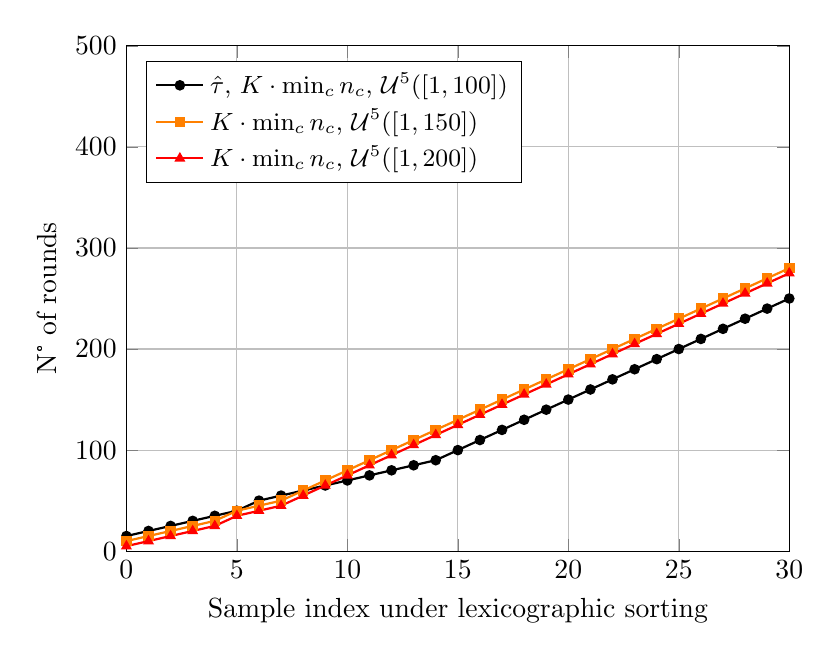
\begin{tikzpicture}
\begin{axis}[
    xlabel={Sample index under lexicographic sorting},
    ylabel={N° of rounds},
    legend pos=north west,
    legend style={font=\small},
    legend cell align={left},
    width=10cm,
    height=8cm,
    xmin=0, xmax=30,
    ymin=0, ymax=500,
    grid=major,
    every axis plot/.append style={thick},
    mark size=1.5
]

% U^5([1,100])
\addplot[color=black, mark=*] coordinates {
    (0, 15) (1, 20) (2, 25) (3, 30) (4, 35) (5, 40) (6, 50) (7, 55) (8, 60) (9, 65) (10, 70)
    (11, 75) (12, 80) (13, 85) (14, 90) (15, 100) (16, 110) (17, 120) (18, 130) (19, 140) (20, 150)
    (21, 160) (22, 170) (23, 180) (24, 190) (25, 200) (26, 210) (27, 220) (28, 230) (29, 240) (30, 250)
};
\addlegendentry{$\hat{\tau}$, $K \cdot \min_c n_c$, $\mathcal{U}^5([1,100])$}

% U^5([1,150])
\addplot[color=orange, mark=square*] coordinates {
    (0, 10) (1, 15) (2, 20) (3, 25) (4, 30) (5, 40) (6, 45) (7, 50) (8, 60) (9, 70) (10, 80)
    (11, 90) (12, 100) (13, 110) (14, 120) (15, 130) (16, 140) (17, 150) (18, 160) (19, 170) (20, 180)
    (21, 190) (22, 200) (23, 210) (24, 220) (25, 230) (26, 240) (27, 250) (28, 260) (29, 270) (30, 280)
};
\addlegendentry{$K \cdot \min_c n_c$, $\mathcal{U}^5([1,150])$};

% U^5([1,200]) - Example data, adjust as per actual data
\addplot[color=red, mark=triangle*] coordinates {
    (0, 5) (1, 10) (2, 15) (3, 20) (4, 25) (5, 35) (6, 40) (7, 45) (8, 55) (9, 65) (10, 75)
    (11, 85) (12, 95) (13, 105) (14, 115) (15, 125) (16, 135) (17, 145) (18, 155) (19, 165) (20, 175)
    (21, 185) (22, 195) (23, 205) (24, 215) (25, 225) (26, 235) (27, 245) (28, 255) (29, 265) (30, 275)
};
\addlegendentry{$K \cdot \min_c n_c$, $\mathcal{U}^5([1,200])$};

% Continue adding plots for other cases in a similar manner...

\end{axis}
\end{tikzpicture}

\end{document}